\documentclass[12pt]{article}

\input{../Tex/header.tex}
%\geometry{twoside,bindingoffset = 2cm,left = 15mm, right = 15mm}
\onehalfspacing
\renewcommand{\bibname}{References}
% opening
\title{PhD Monitoring Report}
\author[1,2]{Samuel  Harrison}
\author[2]{\authorcr Supervisors: Prof. D.T. Papageorgiou}
\author[1]{\authorcr Dr Alex Lukyanov }


\affil[1]{ University of Reading}
\affil[2]{Imperial College London}
\date{\today}

\begin{document}
	\maketitle
	\section{PhD Motivation}
Deposition (e.g. stalagmites and stalactites) and dissolution (e.g. glaciers and icebergs) geomorphic patterns are fundamental in the environment,
and understanding the mechanisms underpinning their formation and evolution is central to paleo-reconstruction techniques used to
probe past climatological systems. Such problems pose numerous mathematical challenges including motion of free boundaries (wall-shape as well
as liquid-air interfaces), fluid-structure interactions and multiscale features in both space and time. The latter can pose particular challenges for
lab experiments (for instance features can form over time scales of hundreds of years) and we propose a complete theoretical approach
to quantify fundamental physical systems in order to compare with field observations.

\section{Proposed Thesis Outline}
Introduction - outlining the literature and motivation of the work. \\
Governing Equations and Scalings - Looking at three main different geometries, to see what affect they have on the fluid thickness.\\
Fluid Thickness Steady States - Seeing how the amplitude and wavelength of the wall disturbance affect the steady fluid thickness. Also looking at varying the Radius of the stalactite, Reynold's number, Bond number and ratio between the fluid thickness and the wavelength of the wall disturbance. In this section we will also look at different shaped walls such as steps and sawtooths.\\
Long Term Behaviour - In this section we numerically simulate the equations for the fluid thickness in order to determine the stability of the steady states, as well as seeing under what conditions periodic solutions and maybe chaotic solutions emerge. \\
Chemistry - In this section we link the fluid thickness to equations for the deposition of calcium on the wall in order to predict the growth of stalactites. \\
Conclusions.
 


\section{Work}
\subsection{Realistic Geometries}
Most of the research previously done on stalactites ignores the cylindrical geometry, treating the stalactite as a flat plate with a film on top \cite{short,camporeale_2017,doi:10.1098/rspa.2015.0031}. While this may give a good approximation for a smooth stalactite, the effects of the cylindrical geometry can not be ignored for when we model the stalactites to have crenulations. This is due to the radius of the stalactite and the wavelength of the crenulations being of similar order. Looking into research about flow down cylinders, many papers take the other extreme. That is making the radius of a comparable length to that of the fluid thickness\cite{ CRASTER_2006}. This method ignores some viscous terms and also some that appear due to the cylindrical geometry. A more realistic geometry for a stalactite can be found in a paper by Frenkel \cite{Frenkel_1992}. Here the radius of the cylinder is of the same order as the vertical length-scale which is much larger than that of the fluid thickness.
\subsection{Scalings}
In order to obtain a more realistic geometry for a stalactite we decided to try different scalings.
Here we started with the Navier Stokes equation in cylindrical coordinates, with no slip; no flux; tangential and normal stress balance; and the kinematic condition. These equations can be found in Appendix \ref{eqs}. The equations were non-dimensionalised using the film thickness as the length-scale and making it a gravity driven flow so that the velocity scales like $W\sim \frac{a_0^2 g}{\nu}$ where $a_0$ is the mean film thickness, $g$ the gravitational constant, and $\nu$ the kinematic viscosity. Then the radial and the downwards spatial components are transformed as such
\begin{align}
\hat{r} = \frac{R}{\epsilon} + \frac{\delta}{\epsilon}\eta(z) + r \\
\hat{z} = \frac{z}{\zeta}
\end{align}
where R is the radius of the stalactite, that for now is treated as a constant. $\eta$ is the shape of the crenulations. $\epsilon , \delta, \zeta$ are small parameters to change the effective size of the radius, crenulation amplitude and crenulation wavelength. Transforming the coordinates like this puts the wall at $r=0$ and the fluid-air interface is at $r = a$. In these schemes we also look at how changing the magnitude of the Reynold's number $\Re = \frac{Ua_0}{\nu}$  and the Bond number $\Bo =\frac{\rho g a_0^2}{\gamma}$ would affect the flow. Changing the size of the Bond number introduces the surface tension into the flow through the pressure term. Changing the size of the Reynolds number can bring the inertia into the flow.
Recent work has focused on the case where $\epsilon = \zeta = \delta$, with the Bond number being order $\frac{1}{\epsilon},\frac{1}{\epsilon^2}$ and the Reynold's number being order 1. This results in the equations
\begin{align}
	h_t + \pdv{z}\left(\frac{h^3}{3}  + \frac{h^3}{3B}\left(\frac{h_z+ \eta_z}{R^2} + h_{zzz}+ \eta_{zzz}\right)\right) = 0\\
	h_t + \pdv{z}\left(\frac{h^3}{3} +\epsilon\left(\frac{2}{15}\Re h^6 h_z + \frac{h^3}{3\Bo}\left(\frac{h_z+ \eta_z}{R^2} + h_{zzz}+ \eta_{zzz}\right)- \frac{h^4}{6R}- \frac{2}{3R}h^3\eta\right)\right)=0\label{maineq}
\end{align}
where $h$ here is the mass density. This has been used instead of the fluid thickness so that the equations are in conservative form. 
 \subsection{Steady States}
 Due to the difference in timescales for calcium deposition and the hydrodynamics, we can treat the fluid as steady \cite{short,PhysRevLett.108.238501}. Since the equation is of the form $h_t + q_x = 0 $, we look for solutions $q = q_0$, where $q_0$ is a constant. To find the fluid thickness we used Matlab's \texttt{fsolve}. Here we looked at the affects that different walls had on the steady state, by varying the wavelenght and the amplitude of sinusoidal walls. We also looked at different shaped walls such as steps and sawtooths. These were smoothed using tanh, however \texttt{fsolve} struggled to find steady states in some of these instances. 
\begin{figure}[H]
	\caption{Example fluid thicknesses with a sinusoidal wall}	\begin{subfigure}{.33\linewidth}
	\centering
	\caption{Varying  the Surface Tension}
	\includegraphics[width =.9\linewidth]{varyBond}
\end{subfigure}	\begin{subfigure}{.33\linewidth}
	\centering
	\caption{Varying the Amplitude}
	\includegraphics[width =.9\linewidth]{varyA}
\end{subfigure}\begin{subfigure}{.33\linewidth}
	\centering
	\caption{Varying the Wavelength}
	\includegraphics[width =.9\linewidth]{varyL}
\end{subfigure}\end{figure}
These figures show the fluid thickness based on the dotted sinusoidal wall.  They show that the fluid is thickest just before the maximum and thinnest just after the maximum. It can also be seen that by increasing the amplitude of the wall, increasing the Bond number, and decreasing the wavelength of the crenulations the fluid thickness increases.

\subsection{Dynamics of the fluid thickness}
We also looked to test the long term behaviour of these steady states, to see if they were stable. Also by integrating this equation we could find steady states that couldn't be picked up by \texttt{fsolve}.
For certain parameters we could find travelling waves, and we wished to see if chaos would form. The equation 
\eqref{maineq} was integrated using Matlab's \texttt{ode45}. Initially the spatial derivatives were calculated using finite differences, however this resulted in a fairly significant loss of mass. Psuedo spectral derivates were later introduced to reduce this error. Animations were made in order to see how the fluid thickness evolved in time. The results were sorted into different categories, whether the fluid thickness went to a steady state, exhibited periodic or quasiperiodic wave patterns. For those that exhibited a travelling wave the wave speed was found. We then looked at how the fluid thickness changed in a frame which moved at this wave speed.
\begin{figure}[H]
	\caption{Example fluid thicknesses with a sinusoidal wall}	\begin{subfigure}{.33\linewidth}
		\centering
		\caption{Energy Norm\newline}
		\includegraphics[width =.9\linewidth,height = .9\linewidth]{/Users/srh18/Documents/PhD/Paper/plots/energyL4pidel2.eps}
	\end{subfigure}	\begin{subfigure}{.33\linewidth}
		\centering
		\caption{Fluid thickness over the \\maximum vs the minimmum}
		\includegraphics[width =.9\linewidth,height = .9\linewidth]{/Users/srh18/Documents/PhD/Paper/plots/Casesn500del1L2pi.eps}
	\end{subfigure}\begin{subfigure}{.33\linewidth}
		\centering
		\caption{Fluid thickness travelling at the wavespeed.}
		\includegraphics[width =.9\linewidth,height = .9\linewidth]{/Users/srh18/Documents/PhD/Paper/plots/ColourL4del1.eps}
\end{subfigure}\end{figure}
These figures look at the Energy norm for a quasiperiodic case, the trajectories over the maxima vs the minima for a periodic orbit, and the fluid thickness if we travel in a frame of reference that follows the wavespeed. In this last figure we can see that for this case it exhibits two modes, which oscillate both in amplitude and position.
\section{Teaching}
I worked as a teaching assistant for year 1 calculus at Imperial College. This involved going through example sheets questions that were set by the lecturer to help with the course. In addition I helped to mark their coursework and mock tests. Additional I marked Vector Calculus for University of Reading.

\section{Met Office Internship}
Over the summer I was working with the Met Office to see whether the impacts from volcanic eruptions would increase or decrease in likelihood according to their climate projections. This was done by looking at the climate through 30 weather patterns that had been derived using k-mean clustering to get a view of different regimes based off their mean sea level pressure. This was then matched to the wind data from 1950-2020, in order to see which regimes would bring ash flow from Iceland. Stream plots were then created to show the mean wind fields of these regimes as an indications of which British airspace the ash would likely impact. The impact was also split into lower level ash flow, to highlight to risk to take off and landing, and higher level ash flow, which affects aeroplanes that would be cruising through these sectors. This was done using python.
\section{Plan for the Year}
\begin{itemize}
\item Write paper on equation (3) November-December
\item Write paper on equation (4) Jan -March
\item Link these papers to the Chemistry March - May
\item Write up thesis June-Oct.
\end{itemize}
\appendix
\section{Equations}
\subsection{Navier Stokes Equation in Cylindrical Coordinates \label{eqs}}

\begin{align}
\pdv{\tilde u}{\tilde r}+\frac{\tilde u}{\tilde r}+\pdv{\tilde w}{\tilde z}&=0\\
\pdv{\tilde u}{\tilde t}+\tilde u\pdv{\tilde u}{\tilde r}+\tilde w\pdv{\tilde u}{\tilde z}&=-\frac{1}{\rho}\pdv{\tilde p}{\tilde r}+\nu\left(\pdv[2]{\tilde u}{\tilde r}+\frac{1}{\tilde r}\pdv{\tilde u}{\tilde r}-\frac{1}{r^2}\tilde u+\pdv[2]{\tilde u}{\tilde z}\right)\\
\pdv{\tilde w}{\tilde t}+\tilde u\pdv{\tilde w}{\tilde r}+\tilde w\pdv{\tilde w}{\tilde z}&=-\frac{1}{\rho}\pdv{\tilde p}{\tilde z}+\nu\left(\pdv[2]{\tilde w}{\tilde r}+\frac{1}{\tilde r}\pdv{\tilde w}{\tilde r}+\pdv[2]{\tilde w}{\tilde z}\right) + g 
\end{align}
\subsection{Boundary Conditions}
\begin{align}
\tilde u=\pdv{\tilde R}{\tilde t},\;\tilde  w=0\quad\mathrm{on}\; \tilde r=\tilde R(\tilde z) 
\end{align}
\begin{align}
\tilde   u=\pdv{\tilde S}{\tilde t}+\tilde w\pdv{\tilde S}{\tilde z} \\
2\pdv{\tilde S}{\tilde z}\left(\pdv{\tilde u}{\tilde r}-\pdv{\tilde w}{\tilde z}\right)+\left(1-\left(\pdv{\tilde S}{\tilde z}\right)^2\right)\left(\pdv{\tilde u}{\tilde z}+\pdv{\tilde w}{\tilde r}\right)&=0\label{tangstress}\\
\tilde p\left(1+\left(\pdv{\tilde S}{\tilde z}\right)^2\right)-2\mu\left( \pdv{\tilde u}{\tilde r}-\pdv{\tilde S}{\tilde z}\left(\pdv{\tilde u}{\tilde z}+\pdv{\tilde w}{\tilde r}\right)+\left(\pdv{\tilde S}{\tilde z}\right)^2\pdv{\tilde w}{\tilde z}\right)&=\gamma\frac{\left(\frac{1}{\tilde S}\left(1+\left(\pdv{\tilde S}{\tilde z}\right)^2\right)-\pdv[2]{\tilde S}{\tilde z}\right)}{\left(1+\left(\pdv{\tilde S}{\tilde z}\right)^2\right)^{\frac{1}{2}}}\label{normstress}
\end{align}

\section{Example Stalactite}
\begin{figure}[H]
	\centering
	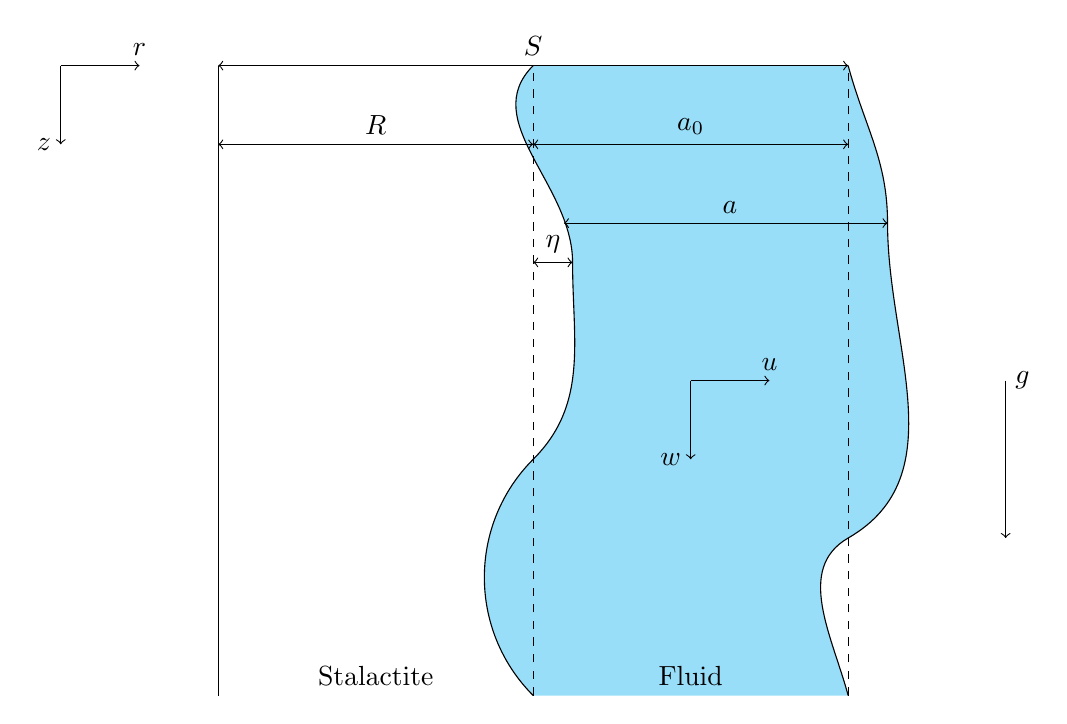
\begin{tikzpicture}
	\draw (0,0) -- (0,8);
	\fill[cyan!40!white] (4,0) to [out=135, in=-135] (4,3) to [out=45,in=-90]  (4.5,5.5) to [out=90,in=-135] (4,8) to (8,8) to [out=-75,in=90] (8.5,6) to [out=-90,in=30] (8,2) to [out=-150,in=105] (8,0) -- cycle;
	\draw[dashed](4,0) -- (4,8);
	\draw[dashed](8,0)--(8,8);
	\draw (4,0) to [out=135, in=-135] (4,3) to [out=45,in=-90]  (4.5,5.5) to [out=90,in=-135] (4,8);
	\draw (8,0) to [out=105, in=-150] (8,2) to [out=30,in=-90]  (8.5,6) to [out=90,in=-75] (8,8);
	\draw[<->](4,5.5)--(4.5,5.5);
	\node[above] at (4.25,5.5) {$\eta$};
	\draw[<->](4.39,6)--(8.5,6);
	\node[above] at (6.5,6) {$a$};
	\draw[<->] (0,7) --(4,7); 
	\node[above] at (2,7) {$R$};
	\draw[<->] (4,7) -- (8,7);
	\node[above] at (6,7) {$a_0$};
	\draw[->] (6,4) --(6,3);
	\node[ left] at (6,3) {$w$};
	\draw[->] (6,4) --(7,4);
	\node[above ] at (7,4) {$ u$};
	\draw[->] (10,4) --(10,2);
	\node[right] at (10,4) {$ g$};
	\draw[<->] (0,8)--(8,8);
	\node[above] at (4,8) {$ S$};
	\node[above] at (2,0) {Stalactite};
	\node[above] at (6,0) {Fluid};
	\draw[->] (-2,8) --(-2,7);
	\node[left] at (-2,7) {$ z$};
	\draw[->] (-2,8) --(-1,8);
	\node[above] at (-1,8) {$ r$};
	\end{tikzpicture}
	\caption{Stalactite with Crenulations\label{sta_cren}}
\end{figure}
\bibliographystyle{plain}
\bibliography{../MRES-Project/Report}
\end{document}